% Introdução

\documentclass[Tese.tex]{subfiles}

\begin{document}
	
\chapter{Termodinâmica e transferência de calor}\label{ch:termodinamica}

Neste capítulo, serão apresentados os conceitos fundamentais da termodinâmica e da transferência de calor, que serão utilizados como base para os modelos termo-mecânicos desenvolvidos neste trabalho.

\section{Primeira lei da termodinâmica}

A primeira lei da termodinâmica, também conhecida como lei da conservação da energia, estabelece que a taxa de energia total de um sistema deve ser nula, isto é:
\begin{equation}\label{eq:1lei}
\dotEnergia = \dotEnergiaint + \dotEnergiacin - \dotEnergiaext - \dotEnergiater = 0 ,
\end{equation}	
onde $\Energiaint$ representa a energia interna do sistema, $\dotEnergiater$ representa o trabalho térmico, e $\Energiacin$ e $\Energiaext$ representam a energia cinética e a energia potencial das forças externas, introduzidas anteriormente pelas \cref{eq:picin,eq:piext}, respectivamente.

A energia interna neste contexto não deve ser confundida com a energia de deformação, apresentada na \cref{eq:pidef}, pois a última abrange apenas a energia que pode ser convertida em trabalho mecânico, não incluindo, por exemplo, parcelas de energia convertidas em rearranjos moleculares ou dissipativas em geral. Define-se a energia interna como:
\begin{equation}\label{eq:piint}
\Energiaint = \int_{\domVoli}\energiaint\,d\voli,
\end{equation}
onde $\energiaint$ é a densidade Lagrangiana de energia interna \textcolor{red}{mudar no restante do texto} (energia interna por unidade de volume na configuração inicial). 

%Vale ser observado que a energia interna específica e outras grandezas apresentadas posteriormente são comumente definidas na literatura por unidade de massa. No entanto, como estamos utilizando uma abordagem totalmente Lagrangiana, optamos por definir essas grandezas por unidade de volume na configuração inicial, quando aplicável. Cabe ressaltar que uma grandeza expressa por unidade de volume na configuração inicial pode ser equivalentemente expressa por unidade de massa, simplesmente dividindo-a pela massa específica do material na configuração inicial ($\massi$).

O trabalho térmico pode ser visto como a quantidade de calor absorvida ou liberada pelo sistema, tanto internamente quanto por meio da superfície de contorno. Assim, podemos defini-lo como:	
\begin{equation}\label{eq:dpiter}
\dotEnergiater = -\boldsymbol{\int}_{\domCon} \q\cdot\normal\,d\con + \int_{\domVoli} \calorInt\,d\voli,
\end{equation}
onde $\q$ é o fluxo de calor aplicado na superfície, $\normal$ é o vetor normal da superfície, e $\calorInt$ é o calor interno gerado por unidade de volume na configuração inicial. Alternativamente, aplicando o teorema da divergência na primeira parcela da \cref{eq:dpiter}, pode-se escrever
\begin{equation}\label{eq:dpiterdiv}
\dotEnergiater = -\int_{\domVol} \gradiente\cdot\q\,d\vol + \int_{\domVoli} \calorInt\,d\voli.
\end{equation}

Nas \cref{eq:dpiter,eq:dpiterdiv}, $\q$ e $\normal$ são definidos na configuração atual. Para obter uma versão totalmente Lagrangiana do trabalho térmico, podemos utilizar a fórmula de Nanson -- \cref{eq:mudanca-area} --, que resulta em
\begin{equation}\label{eq:q00}
\q\cdot(\normal\,d\con) = \q\cdot(\J\F^{-T}\cdot\normali\,d\coni) = (\J\F^{-1}\cdot\q)\cdot \normali\, d\coni,
\end{equation}
onde $\normali$ é o vetor normal da superfície na configuração inicial. Define-se, portanto, o fluxo de calor na configuração inicial como
\begin{equation}\label{eq:q0}
\qi = \J\F^{-1}\cdot\q.
\end{equation}		
Aplicando-se as \cref{eq:q00,eq:q0} na \cref{eq:dpiter}, escrevemos o trabalho térmico em sua forma Lagrangiana como:	
\begin{equation}\label{eq:dpiter0}
\dotEnergiater = -\int_{\domConi} \qi\cdot\normali\,d\coni + \int_{\domVoli}\calorInt\,d\voli.
\end{equation}
Utilizando novamente o teorema da divergência, isso resulta em:
\begin{equation}\label{eq:dpiter1}
\dotEnergiater = -\int_{\domVoli} \gradientei\cdot\qi\,d\voli + \int_{\domVoli}\calorInt\,d\voli.
\end{equation}

Os valores de $\dotEnergiaint$, $\dotEnergiacin$ e $\dotEnergiaext$ podem ser facilmente calculados pelas equações \eqref{eq:piint}, \eqref{eq:picin} e \eqref{eq:piext}. Ao aplica-los juntamente com a \cref{eq:dpiter1} na \cref{eq:1lei}, pode-se expressar a primeira lei da termodinâmica em sua forma Lagrangiana como:
\begin{equation}
\begin{aligned}\label{eq:primeira-lei}
\dotEnergia = & \overbrace{\int_{\domVoli}\dotenergiaint\,d\voli}^\text{Parcela interna} + \overbrace{\int_{\domVoli}\massi \ddoty\cdot\doty\,d\voli}^\text{Parcela cinética} - \overbrace{\int_{\domConi}\mathbf{p}\cdot\doty\,d\coni - \int_{\domVoli}\mathbf{b}\cdot\doty\,d\voli}^\text{Parcela das forças externas}  \\
& + \underbrace{\int_{\domVoli} \gradientei\cdot\qi\,d\voli - \int_{\domVoli}\calorInt\,d\voli}_\text{Parcela térmica} = 0.
\end{aligned}
\end{equation}

Uma forma mais conveniente da \cref{eq:primeira-lei} pode ser obtida com a aplicação do princípio da taxa de trabalho \textcolor{red}{(colocar referência para esse princípio)}. Tal princípio estabelece que a taxa da energia cinética é igual à taxa do trabalho das forças externas e internas. Utilizando as equações \eqref{eq:dpidef}, \eqref{eq:dpicin} e \eqref{eq:dpiext}, temos:
\begin{equation}
\int_{\domVoli}\massi \ddoty\cdot\doty\,d\voli = \int_{\domConi}\mathbf{p}\cdot\doty\,d\coni + \int_{\domVoli}\mathbf{b}\cdot\doty\,d\voli - \int_{\domVoli}\S:\dotE\,d\voli.
\end{equation}
Aplicando na \cref{eq:primeira-lei}, escreve-se a primeira lei da termodinâmica como:
\begin{equation}%\label{eq:primeira-lei}
\dotEnergia = \int_{\domVoli}\dotenergiaint\,d\voli - \int_{\domVoli}\S:\dotE\,d\voli + \int_{\domVoli} \gradientei\cdot\qi\,d\voli - \int_{\domVoli} \calorInt\,d\voli = 0.
\end{equation}
Pela arbitrariedade do volume, podemos ainda expressa-la na seguinte forma local Lagrangiana:
\begin{equation}\label{eq:primeira-lei-local}
\dotenergiaint - \calorInt = \S:\dotE - \gradientei\cdot\qi.
\end{equation}

\section{Segunda lei da termodinâmica}

O conceito de entropia foi estabelecido originalmente em 1865 pelo físico alemão Rudolf Clausius, com origens na palavra grega que significa ``transformação''. A entropia pode ser entendida como um número que mede a desordem do sistema termodinâmico, sendo associada à quantidade de energia que não pode ser convertida em trabalho.

A segunda lei da termodinâmica afirma que a quantidade de entropia de um sistema isolado sempre tende a aumentar até alcançar um valor máximo, no qual ocorre o equilíbrio termodinâmico. Uma das bases dessa lei se deve a Clausius, que afirmou, a partir de seus estudos, que o calor não pode passar de um corpo mais frio para um mais quente de forma espontânea. Essa lei, portanto, trata da irreversibilidade dos processos naturais, explicando fenômenos, como atrito e dissipação, que não são abrangidos pela primeira lei da termodinâmica.

Matematicamente, existem diversas maneiras de expressar a segunda lei da termodinâmica, sendo uma das mais utilizadas no contexto da mecânica do contínuo a inequação de Clausius-Duhem, dada em sua forma Lagrangiana por
\begin{equation}\label[ineq]{eq:segunda-lei-0}
\displaystyle\int_{\domVoli}\dotentropy\,d\voli \geq \int_{\domVoli} \dfrac{\calorInt}{\temp}\,d\voli - \int_{\domConi} \dfrac{\qi\cdot\normali}{\temp}\,d\coni,
\end{equation}
onde $\entropy$ representa a entropia por unidade de volume na configuração inicial, e $\temp$ a temperatura absoluta. Levando em conta o teorema da divergência na última parcela da \cref{eq:segunda-lei-0}, é possível expressar a integral no contorno por uma integral no volume, isto é:
\begin{equation}\label[ineq]{eq:segunda-lei-1}
\displaystyle\int_{\domVoli}\dotentropy\,d\voli \geq \int_{\domVoli} \dfrac{\calorInt}{\temp}\,d\voli - \int_{\domVoli} \gradientei\cdot\left(\dfrac{\qi}{\temp}\right)\,d\voli,
\end{equation}
de onde, pela arbitrariedade do volume, segue que:
\begin{equation}\label[ineq]{eq:segunda-lei-local-0}
\dotentropy \geq \dfrac{\calorInt}{\temp} - \gradientei\cdot\left(\dfrac{\qi}{\temp}\right).
\end{equation}
Desenvolvendo algebricamente, escreve-se:
\begin{equation}\label[ineq]{eq:segunda-lei-local-1}
\temp \dotentropy \geq \calorInt - \gradientei\cdot\qi + \dfrac{1}{\temp}\qi\cdot\gradientei\,\temp.
\end{equation}
Finalmente, aplicando-se a forma local da primeira lei da termodinâmica, dada na \cref{eq:primeira-lei-local}, a inequação de Clausius-Duhem pode ser expressa na seguinte forma local Lagrangiana:
\begin{equation}\label[ineq]{eq:clausius-duhem-0}
\dissipation = \S:\dotE + \temp \dotentropy - \dotenergiaint - \dfrac{1}{\temp}\qi\cdot\gradientei\,\temp \geq 0.
\end{equation}
onde $\dissipation$ representa a taxa de dissipação interna por unidade de volume na configuração inicial. % Definida como a taxa de produção interna de entropia vezes a temperatura absoluta (ver https://en.wikipedia.org/wiki/Clausius%E2%80%93Duhem_inequality) 

\section{Energia livre de Helmholtz}

A energia livre de Helmholtz, já apresentada na \autoref{subsec:energiadef}, pode ser entendida como a parcela da energia interna específica efetivamente convertida em trabalho mecânico, sendo utilizada para definir o modelo constitutivo do material. Essa é definida, por unidade de volume na configuração inicial, como:
\begin{equation}\label{eq:helmholtz}
\helmholtz = \energiaint - \temp\entropy.
\end{equation}
A partir dessa definição, temos que
\begin{equation}\label{eq:dothelmholtz}
\dothelmholtz = \dotenergiaint- \temp \dotentropy - \dottemp {\entropy}.
\end{equation}
Aplicando essa expressão em \cref{eq:primeira-lei-local,eq:clausius-duhem-0}, pode-se escrever a primeira e segunda lei da termodinâmica em termos da energia livre de Helmholtz como:
\begin{align}
& \dothelmholtz + \temp \dotentropy + \dottemp {\entropy} - \calorInt = \S:\dotE - \gradientei\cdot\qi, \label{eq:primeira-lei-2} \\
&\dissipation = \S:\dotE - \dothelmholtz - \dottemp {\entropy} - \dfrac{1}{T}\qi\cdot\gradientei\,\temp \geq 0. \label[ineq]{eq:clausius-duhem}
\end{align}

A \cref{eq:clausius-duhem} é utilizada neste trabalho para garantir que os modelos constitutivos sejam termodinamicamente consistentes, sendo aplicada inclusive em problemas isotérmicos, nos quais ela é reduzida a
\begin{equation}
\dissipation = \S:\dotE - \dothelmholtz \geq 0. \label[ineq]{eq:clausius-duhem-iso}
\end{equation}
A partir disso, é possível mostrar que modelos hiperelásticos isotérmicos não provocam dissipação, uma vez que a energia livre de Helmholtz, nesse caso, depende apenas da deformação, e, portanto,
\begin{equation}
\dothelmholtz = \dfrac{\partial \helmholtz}{\partial \E}:\dotE = \S:\dotE,
\end{equation}
provando que $\dissipation=0$.

\section{Equação da condução de calor}\label{sec:conducao-calor-0}

\textcolor{red}{Precisa ficar claro se precisa V0 precisa ser igual a Vf ou se o que você está considerando é um problema de condução de calor em um domínio com deformação independente do problema térmico.}

Considerando problemas puramente térmicos, onde desprezam-se os efeitos mecânicos, a energia livre de Helmholtz pode ser expressa como função apenas da temperatura, isto é, $\helmholtz = \helmholtz(\temp)$. Assim, temos:
\begin{equation}
\dothelmholtz = \dfrac{\partial\helmholtz}{\partial\temp}\dottemp.
\end{equation}
Além disso, é possível desconsiderar os termos $\S:\dotE$ da \cref{eq:primeira-lei-2} e da  \cref{eq:clausius-duhem}. Dessa forma, essas podem ser escritas como:
\begin{align}
&\left(\dfrac{\partial \helmholtz}{\partial \temp} + {\entropy}\right)\dottemp  + \temp \dotentropy - \calorInt + \gradientei\cdot\qi = 0, \label{eq:primeira-lei-mod0} \\
&\dissipation = - \left(\dfrac{\partial \helmholtz}{\partial \temp} + {\entropy}\right)\dottemp - \dfrac{1}{T}\qi\cdot\gradientei\,\temp \geq 0. \label[ineq]{eq:clausius-duhem-mod0}
\end{align}

Uma vez que $\dottemp$ é arbitrário, é necessário que seu termo multiplicante seja nulo para que as leis da termodinâmica sejam atendidas. Assim, a seguinte expressão para a entropia é obtida:
\begin{equation}
\entropy=-\dfrac{\partial \helmholtz}{\partial \temp},\label{eq:const2-0} 
\end{equation}
que reduz as leis da termodinâmica às seguintes expressões:
\begin{align}{ }
&
\temp \dotentropy - \calorInt + \gradientei\cdot\qi = 0, \label{eq:cond0-0}
\\[0.1cm]
&
\qi\cdot\gradientei\,\temp \leq 0. \label[ineq]{eq:cond-termo-0}
\end{align}

A \cref{eq:cond0-0} é denominada equação da condução de calor, expressa nesse contexto em sua forma simplificada para o caso puramente térmico. A taxa de entropia pode ser calculada a partir da \cref{eq:const2-0} como
\begin{equation}\label{eq:dotentropy-0}
\dotentropy = -\dfrac{\partial^2 \helmholtz}{\partial \temp^2}\dottemp = \dfrac{\volumetricHeatCapacity}{\temp}\dottemp = \massi\dfrac{\specificHeat}{\temp}\dottemp,
\end{equation}
onde $\volumetricHeatCapacity$ é o calor específico volumétrico do material, definido por unidade de volume na configuração inicial a partir da expressão
\begin{equation}\label{eq:specific-heat}
\volumetricHeatCapacity = -\temp\dfrac{\partial^2 \helmholtz}{\partial \temp^2} = \temp\dfrac{\partial\entropy}{\partial\temp},
\end{equation}
e $\specificHeat$ é o calor específico por unidade de massa, que pode ser associado ao calor específico volumétrico pela relação $\volumetricHeatCapacity = \massi\specificHeat$. Ambos são formas alternativas de expressar a mesma grandeza. Embora o calor específico por unidade de massa seja mais comumente utilizado na literatura, adotaremos predominantemente $\volumetricHeatCapacity$ ao longo deste trabalho, para manter a abordagem totalmente Lagrangiana.

\textcolor{red}{$c_v$ é muito utilizado para calor específico a volume contante. Pode ser interessante mudar a variável...}
Em geral, o calor específico é um parâmetro do material que pode ser constante ou variar em função da temperatura. Considerando um caso no qual ele varia linearmente com relação à temperatura, podemos definir a energia livre de Helmholtz pela expressão dada em \citeonline{vujovsevic2002finite}:
\begin{equation}\label{eq:helmholtz-t-0}
\helmholtz(\temp) = (\specificHeatIni-\specificHeatConst\tempref)\left(\temp-\tempref-\temp \ln{\dfrac{\temp}{\tempref}}\right)-\dfrac{1}{2}\specificHeatConst(\temp-\tempref)^2,
\end{equation}
onde $\tempref$ é a temperatura de referência do material, $\specificHeatIni$ é uma constante de referência para o calor específico,  e $\specificHeatConst$ é um parâmetro que controla a variação do calor específico volumétrico com relação à temperatura. Assim, tem-se:
\begin{align}
&\entropy = -\dfrac{\partial \helmholtz}{\partial \temp} = -(\specificHeatIni-\specificHeatConst\tempref)\ln\left(\dfrac{\tempref}{\temp}\right)+\specificHeatConst(\temp-\tempref), \\[0.1cm]
&\volumetricHeatCapacity = \temp\dfrac{\partial\entropy}{\partial\temp} = \specificHeatIni+\specificHeatConst(\temp - \tempref). \label{eq:calor-especifico-0}
\end{align}

Aplicando a \cref{eq:dotentropy-0} na \cref{eq:cond0-0}, obtém-se:
\begin{equation}\label{eq:equacao-conducao-local-0}
\gradientei\cdot\qi + \volumetricHeatCapacity\dottemp - \calorInt = 0,
\end{equation}
que representa a equação da condução de calor em sua forma local. Essa pode ainda ser escrita em forma variacional ao ser multiplicada por uma função ponderadora $\delta\temp$, isto é:
\begin{equation}\label{eq:equacao-conducao-variacional-0}
\left(\gradientei\cdot\qi + \volumetricHeatCapacity\dottemp - \calorInt\right)\delta\temp = 0.
\end{equation}
Além disso, integrando-a no volume inicial, pode-se escreve-la na forma global:
\begin{equation}\label{eq:equacao-conducao-global-0-0}
\int_{\domVoli}\left(\gradientei\cdot\qi\right)\delta\temp d\voli + \int_{\domVoli}\volumetricHeatCapacity\dottemp\delta\temp d\voli - \int_{\domVoli} \calorInt\delta\temp d\voli = 0.
\end{equation}
Pela regra do produto, tem-se que $\gradientei\cdot\left(\qi\,\delta\temp\right) = \left(\gradientei\cdot\qi\right)\delta\temp + \qi\cdot\left(\gradientei\,\delta\temp\right)$. Logo, o primeiro termo da \cref{eq:equacao-conducao-global-0-0} pode ser reescrito como:
\begin{equation}\label{eq:eq-cond-termo1-0}
\int_{\domVoli}\left(\gradientei\cdot\qi\right)\delta\temp d\voli = - \int_{\domVoli}\qi\cdot\left(\gradientei\,\delta\temp\right) d\voli + \int_{\domVoli}\gradientei\cdot\left(\qi\,\delta\temp\right) d\voli.
\end{equation}
Aplicando-se o teorema da divergência no último termo da \cref{eq:eq-cond-termo1-0} resulta:
\begin{equation}\label{eq:eq-cond-termo1-2-0}
\int_{\domVoli}\gradientei\cdot\left(\qi\,\delta\temp\right) d\voli = \int_{\domConi}\qi\cdot\normali\,\delta\temp d\coni = \int_{\domConi}\qpresci\,\delta\temp d\coni,
\end{equation}
onde $\qpresci = \qi\cdot\normali$ denota o calor prescrito no contorno do corpo, definido por unidade de área na configuração inicial. Aplicando-se, enfim, as \cref{eq:eq-cond-termo1-0,eq:eq-cond-termo1-2-0} na \cref{eq:equacao-conducao-global-0-0}, é possível expressar a equação da condução de calor em sua forma variacional global como:
\begin{equation}\label{eq:equacao-conducao-global-02}
\int_{\domVoli}\qi\cdot\left(\gradientei\,\delta\temp\right) d\voli = \int_{\domVoli}\volumetricHeatCapacity\dottemp\delta\temp d\voli + \int_{\domConi}\qpresci\,\delta\temp d\coni - \int_{\domVoli}\calorInt\delta\temp d\voli.
\end{equation}

%Pela relação \eqref{eq:q00}, o termo de calor prescrito no contorno da \cref{eq:equacao-conducao-global-02} pode ser reescrito em forma Euleriana como:
%\begin{equation}
%\int_{\domConi}\qpresci\,\delta\temp d\coni = \int_{\domCon}\qpresc\,\delta\temp d\con,
%\end{equation}
%onde $\qpresc = \q\cdot\normal$ é o calor prescrito no contorno do corpo, definido por unidade de área na configuração deformada.

É importante destacar que a \cref{eq:equacao-conducao-global-02} é deduzida para o caso puramente térmico. Em casos onde considera-se o acoplamento termo-mecânico, termos adicionais devem ser introduzidos, a depender do modelo constitutivo considerado. Mais detalhes sobre esses termos serão apresentados em capítulos posteriores.

\subsection{Lei de Fourier}\label{subsec:fourier-0}

Para que a condição \eqref{eq:cond-termo-0} seja atendida, o fluxo de calor deve ser tomado como uma função no mínimo linear do gradiente da temperatura. Essa relação é estabelecida pela lei de Fourier, escrita em forma Lagrangiana como:
\begin{equation}\label{eq:fourier-0-term}
\qi = -\condutMati\cdot\gradientei\,\temp,
\end{equation}
onde $\condutMati$ é a matriz de condutividade térmica do material definida na configuração inicial. Utilizando a relação entre $\q$ e $\qi$ estabelecida pela \cref{eq:q0}, e a identidade $\gradiente\temp = \F^{-T}\cdot\gradientei\,\temp$, pode-se escrever a lei de Fourier também na forma Euleriana:
\begin{equation}\label{eq:fourier-term}
\q = -\condutMat\cdot\gradiente\temp,
\end{equation}
onde $\condutMat$, denominada a matriz de condutividade térmica do material na configuração deformada, relaciona-se com $\condutMati$ pela expressão:
\begin{equation}\label{eq:relacao-condut-term}
\condutMati = \J \F^{-1}\cdot\condutMat\cdot\F^{-T}.
\end{equation}

Da \cref{eq:relacao-condut-term}, segue que as matrizes $\condutMat$ e $\condutMati$ não podem ser simultaneamente independentes das deformações, isto é, caso uma seja tomada constante, a outra irá variar em função de $\F$. Naturalmente, a questão sobre qual delas, ou sequer alguma delas, pode ser tomada constante, irá depender do material sendo tratado. No entanto, observa-se que, tomando $\condutMati$ constante, o primeiro termo da \cref{eq:equacao-conducao-global-02} se torna totalmente independente da configuração atual, isto é, o material poderia deformar-se indefinidamente sem causar influência no problema térmico. Embora isso simplifique as equações, o seu sentido físico pode ser questionado. Dessa forma, opta-se por tomar a matriz Euleriana $\condutMat$ independente das deformações. Em geral, essa poderia variar com a temperatura, porém, isso não é considerado neste trabalho. Assumindo ainda o caso isotrópico, pode-se escrever 
\begin{equation}
\condutMat=\condut\I,
\end{equation}onde $\condut$ é uma constante única de condutividade térmica, tomada sempre positiva para que a \cref{eq:cond-termo} seja atendida. Aplicando essa lei isotrópica na \cref{eq:relacao-condut-term}, pode-se obter a matriz Lagrangiana pela expressão 
\begin{equation}\label{eq:condutMat-term}
\condutMati = \condut J \C^{-1}. 
\end{equation}

A equação da condução de calor, \eqref{eq:equacao-conducao-global-02}, pode ser então reescrita substituindo a \cref{eq:fourier-0-term} no primeiro termo:
\begin{equation}\label{eq:equacao-conducao-global-fourier-term}
\int_{\domVoli}\left(\condutMati\cdot\gradientei\,\temp\right)\cdot\left(\gradientei\,\delta\temp\right) d\voli + \int_{\domVoli}\volumetricHeatCapacity\dottemp\delta\temp d\voli + \int_{\domConi}\qpresci\,\delta\temp d\coni - \int_{\domVoli} \calorInt\delta\temp d\voli = 0.
\end{equation}
Pode-se verificar ainda que, a partir das relações apresentadas,
\begin{equation}\label{eq:relacao-condut-int-term}
\int_{\domVoli}\left(\condutMati\cdot\gradientei\,\temp\right)\cdot\left(\gradientei\,\delta\temp\right) d\voli = \int_{\domVol}\left(\condutMat\cdot\gradiente\,\temp\right)\cdot\left(\gradiente\,\delta\temp\right) d\vol,
\end{equation}
isto é, o primeiro termo da \cref{eq:equacao-conducao-global-fourier-term} pode ser calculado tanto em forma Lagrangiana quanto Euleriana sem haja necessidade de reformular os demais termos da equação.

\subsection{Condição de convecção}

\textcolor{red}{Tente entender bem essa condição. Note que só há convecção (transporte junto com a matéria) no fluido que está ao redor do sólido...}

A condição de contorno de convecção é utilizada para representar a troca de calor com o ambiente efetuada por meio da movimentação dos fluidos externos, como, por exemplo, o ar. Utilizando a lei de resfriamento de Newton, temos:
\begin{equation}
\qpresc = \constResfriamento(\temp-\tempext),
\end{equation}
onde $\constResfriamento$ é o coeficiente de transferência de calor por convecção, ou coeficiente de resfriamento, definido por unidade de área na configuração deformada, e $\tempext$ é a temperatura do ambiente externo. Assim, nos contornos do corpo onde ocorre a convecção, o seguinte termo é adicionado à equação da condução de calor:
\begin{equation}
\int_{\domCon}\qpresc\,\delta\temp d\con = \int_{\domCon}\constResfriamento(\temp-\tempext)\delta\temp d\con.
\end{equation}
Assim, a equação da condução de calor pode ser reescrita como:
\begin{equation}\label{eq:equacao-conducao-global-convec-term}
\begin{aligned}
&\int_{\domVoli}\left(\condutMati\cdot\gradientei\,\temp\right)\cdot\left(\gradientei\,\delta\temp\right) d\voli + \int_{\domVoli}\volumetricHeatCapacity\dottemp\delta\temp d\voli + \int_{\domConi}\qpresci\,\delta\temp d\coni \\& + \int_{\domConConv}\constResfriamento(\temp-\tempext)\delta\temp d\con - \int_{\domVoli} \calorInt\delta\temp d\voli  = 0.
\end{aligned}
\end{equation}
onde $\domConConv$ representa o contorno onde aplicam-se as condições de convecção. Observa-se que o termo de convecção da \cref{eq:equacao-conducao-global-convec-term} é integrado na configuração deformada, ao contrário dos demais.

\section{Método dos elementos finitos aplicado ao problema térmico}\label{sec:mef-termo}

Assim como no problema mecânico, utiliza-se neste trabalho o método dos elementos finitos para resolver numericamente o problema térmico. Os conceitos básicos do método, como as funções de forma e a discretização espacial, podem ser aproveitados do problema mecânico, conforme descrito na \autoref{sec:mef}. 

No caso térmico, os parâmetros nodais a serem calculados são as temperaturas. Assim, no domínio de um elemento finito, pode-se realizar a seguinte interpolação:
\begin{equation}\label{eq:interp-temp}
\temp=\fforma\nodeind\temp\nodeind,
\end{equation}
onde $\temp\nodeind$ representa a temperatura no nó $\node$, e os índices $\node$ são somados por todos os nós do elemento. Ainda, pelo método de Galerkin, pode-se escrever
\begin{equation}\label{eq:interp-dtemp}
\delta\temp=\fforma\nodeind\delta\temp\nodeind,
\end{equation}
onde $\delta\temp\nodeind$ representa os valores nodais das funções ponderadoras.

Aplicando as \cref{eq:interp-temp,eq:interp-dtemp} na \cref{eq:equacao-conducao-global-convec-term}, e considerando a isotropia do material, escreve-se a equação da condução de calor como:
\begin{equation}\label{eq:conducao-mef-0}
\begin{aligned}
&\int_{\domVoli}\condut\J\left(\C^{-1}\cdot\gradientei\,\fforma\nodeindDois\right)\cdot\left(\gradientei\,\fforma\nodeind\right)\temp\nodeindDois\delta\temp\nodeind d\voli + \int_{\domVoli}\volumetricHeatCapacity\fforma\nodeind\fforma\nodeindDois\dottemp\nodeindDois\delta\temp\nodeind d\voli \\&+ \int_{\domConi}\qpresci\fforma\nodeind\delta\temp\nodeind d\coni  + \int_{\domConConv}\constResfriamento(\fforma\nodeindDois\temp\nodeind-\tempext)\fforma\nodeind\delta\temp\nodeind d\con - \int_{\domVoli} \calorInt\fforma\nodeind\delta\temp\nodeind d\voli  = 0.
\end{aligned}
\end{equation}
Pela arbitrariedade de $\delta\temp\nodeind$, a \cref{eq:conducao-mef-0} implica que, para cada nó $\node$, deve valer:
\begin{equation}\label{eq:conducao-mef-1}
\begin{aligned}
&\int_{\domVoli}\condut\J\left(\C^{-1}\cdot\gradientei\,\fforma\nodeindDois\right)\cdot\left(\gradientei\,\fforma\nodeind\right)\temp\nodeindDois d\voli + \int_{\domVoli}\volumetricHeatCapacity\fforma\nodeind\fforma\nodeindDois\dottemp\nodeindDois d\voli + \int_{\domConi}\qpresci\fforma\nodeind d\coni\\&  + \int_{\domConConv}\constResfriamento(\fforma\nodeindDois\temp\nodeindDois-\tempext)\fforma\nodeind d\con - \int_{\domVoli} \calorInt\fforma\nodeind d\voli  = 0,
\end{aligned}
\end{equation}
o que nos fornece $N$ equações, onde $N$ é o número de nós da discretização. Esse sistema pode ser organizado globalmente como:
\begin{equation}\label{eq:sistema-termo-0}
\matC\cdot\vetDotTemp + \matK\cdot\vetTemp = \vetF ,
\end{equation}
onde $\vetTemp$ representa o vetor de parâmetros nodais, e:
\begin{align}
&\matC_{ij} = \int_{\domVoli}\volumetricHeatCapacity\fforma^i\fforma^j d\voli, \label{eq:matC}\\[0.1cm]
&\matK_{ij} = \int_{\domVoli}\condut\J\left(\C^{-1}\cdot\gradientei\,\fforma^j\right)\cdot\left(\gradientei\,\fforma^i\right) d\voli + \int_{\domConConv}\constResfriamento\fforma^i\fforma^j d\con, \label{eq:matK} \\[0.1cm]
&\vetF_{i} = -\int_{\domConi}\qpresci\fforma^i d\coni + \int_{\domConConv}\constResfriamento\tempext\fforma^i d\con + \int_{\domVoli} \calorInt\fforma^i d\voli. \label{eq:vetF}
\end{align}

Tendo em vista que as funções de forma são definidas em coordenadas adimensionais, os termos $\gradientei\,\fforma^i$ na \cref{eq:matK} podem ser calculados da seguinte maneira:
\begin{equation}\label{eq:gradientei-fforma}
\gradientei\,\fforma^i = \dfrac{\partial\fforma^i}{\partial\coords}\cdot\dfrac{\partial\coords}{\partial\x} = \dfrac{\partial\fforma^i}{\partial\coords}\cdot\Fini^{-1} = \Fini^{-T}\cdot\dfrac{\partial\fforma^i}{\partial\coords},
\end{equation}
onde $\Fini$ é definido conforme a \cref{eq:F0}.

Alternativamente, o termo da condutividade térmica pode ser calculado pela abordagem Euleriana, utilizando a relação dada na \cref{eq:relacao-condut-int-term}. Dessa forma, podemos escrever:
\begin{equation}
\matK_{ij} = \int_{\domVol}\condut\left(\gradiente\,\fforma^j\right)\cdot\left(\gradiente\,\fforma^i\right) d\vol + \int_{\domConConv}\constResfriamento\fforma^i\fforma^j d\con,  \\[0.1cm]
\end{equation}
onde, de maneira análoga à \cref{eq:gradientei-fforma}, temos:
\begin{equation}\label{eq:gradiente-fforma}
\gradiente\,\fforma^i = \dfrac{\partial\fforma^i}{\partial\coords}\cdot\dfrac{\partial\coords}{\partial\y} = \dfrac{\partial\fforma^i}{\partial\coords}\cdot\Ffin^{-1} = \Ffin^{-T}\cdot\dfrac{\partial\fforma^i}{\partial\coords},
\end{equation}
sendo $\Ffin$ definido conforme a \cref{eq:F1}.

Para que o sistema da \cref{eq:sistema-termo-0} possa ser resolvido numericamente, resta definir como será tratada a taxa dos parâmetros nodais, $\vetDotTemp$. Neste trabalho, utiliza-se o método de Euler, também conhecido como método implícito, ou \emph{backward Euler}, no qual escreve-se:\begin{equation}
\vetDotTemp = \dfrac{1}{\Delta t}\left(\vetTemp - \vetTempAnt\right),
\end{equation}
onde $\vetTempAnt$ denota os parâmetros nodais no passo anterior da análise, e $\Delta t$ é o intervalo de tempo entre os passos. Assim, pode-se reescrever a \cref{eq:sistema-termo-0} como:
\begin{equation}\label{eq:conducao-final}
\left(\Delta t^{-1}\matC + \matK\right)\cdot\vetTemp = \vetF + \Delta t^{-1}\matC\cdot\vetTempAnt,
\end{equation}
resultando em um sistema linear para $\vetTemp$.

\textcolor{red}{Um questionamento bem forte que pode surgir aqui é porque você usou um método de primeira ordem e altamente dissipativo no tempo (backward Euler), se você poderia ter utilizado Newmark, alpha generalizado, diferenças centrais, trapézios... que são métodos de segunda ordem e menos dissipativos. Apenas esteja preparado para isso.}

\subsection{Exemplo numérico: problema puramente térmico}\label{subsec:exemplo-termo}

Este exemplo é proposto para verificar o modelo térmico implementado. O problema consiste de um cubo com dimensões unitárias, sujeito a temperaturas prescritas nas bordas superior e inferior, fluxo de calor prescrito na borda direita e condição de convecção da borda esquerda. Realiza-se uma análise transiente, com carregamentos térmicos constantes ao longo do tempo. Os dados relativos às características físicas, condições de contorno e discretização adotados estão dispostos na \autoref{fig:exemplo-termo}.

\begin{figure}[!htb]
	\centering
	\caption{Dados do exemplo puramente térmico}
	\label{fig:exemplo-termo}
	{\small
		\noindent\shadowbox{
			\parbox{15.3cm}{
				\setlength{\columnseprule}{1pt}
				\vspace{-0.4cm}
				{\centering\begin{center}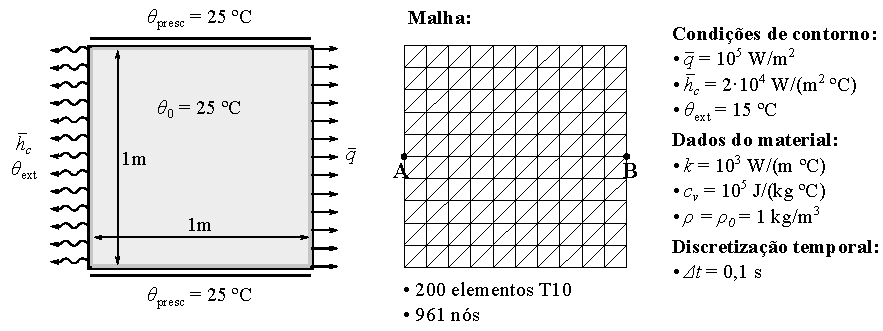
\includegraphics[scale=1.02]{Figuras/ThermoExample1/ThermoExample.pdf}\end{center}\par}
				\vspace{-0.4cm}
			}
		}
	}	
	%\caption*{\textbf{Fonte:} Elaborado pelo autor}
\end{figure}

Os resultados são comparados com resultados obtidos pelo \emph{software} ANSYS, mostrando excelente concordância conforme atestam as \cref{fig:thermo1-comparacao,fig:termo-ABC,fig:ThermoExamplePath}. Na \autoref{fig:thermo1-comparacao}, compara-se qualitativamente os campos de temperatura no instante final da análise ($t=100\,$s). Na \autoref{fig:termo-ABC}, são traçados os gráficos de temperatura ao longo do tempo para os pontos A e B indicados na \autoref{fig:exemplo-termo}. Por fim, na \autoref{fig:ThermoExamplePath} são mostrados os gráficos de temperatura ao longo de um eixo $x$ horizontal, com origem no ponto A, para diversos instantes ao longo da análise.

\begin{figure}[!htb]
	\centering
	\caption{Coomparação entre os campos de temperatura obtidos neste trabalho (à esquerda) e no \emph{software} ANSYS (à direita) para o tempo de análise $100$s.}
	\label{fig:thermo1-comparacao}
	\includegraphics[scale=0.35]{Figuras/ThermoExample1/Thermo1-comparacao.png}
	%\caption*{\textbf{Fonte:} Elaborado pelo autor}
\end{figure}
\begin{figure*}[!b]
	\centering
	\caption{Temperatura (em $^{\circ}$C) ao longo do tempo nos pontos A e B do exemplo puramente térmico.}
	\label{fig:termo-ABC}
	\makebox[\textwidth]{
		\captionsetup[subfigure]{aboveskip=-0.6pt,belowskip=-0.7pt}
		\begin{subfigure}{8.4cm}
			\centering
			\subcaption{}
			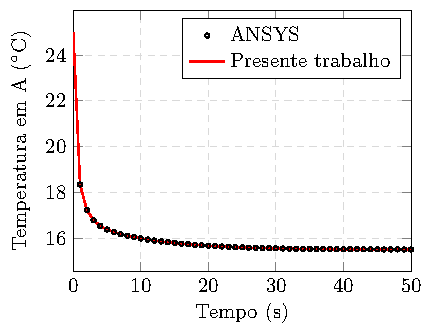
\includegraphics[scale=1.08]{Figuras/ThermoExample1/A.pdf}			
		\end{subfigure}%7
		\begin{subfigure}{8.4cm}
			\centering
			\subcaption{}
			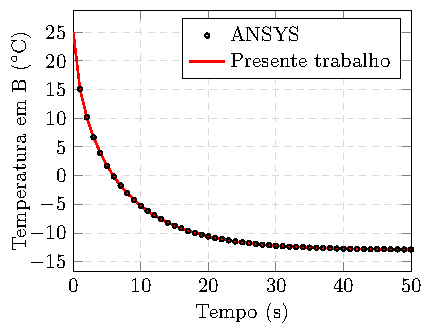
\includegraphics[scale=1.08]{Figuras/ThermoExample1/B.pdf}			
		\end{subfigure}
	}		
	%\caption*{\textbf{Fonte:} Elaborado pelo autor}
\end{figure*}
\begin{figure}[!htb]
	\centering
	\caption{Temperatura ao longo do eixo horizontal que percorre os pontos A e B em diversos tempos de análise para o exemplo puramente térmico}
	\label{fig:ThermoExamplePath}
	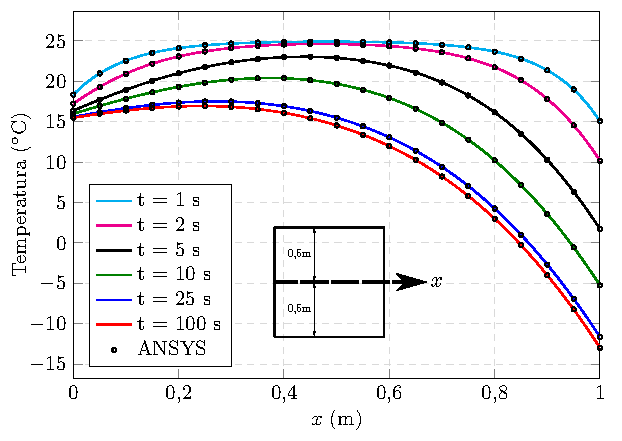
\includegraphics[scale=1.05]{Figuras/ThermoExample1/ThermoExamplePath.pdf}
	%\caption*{\textbf{Fonte:} Elaborado pelo autor}
\end{figure}

%\newpage
%\null
%\vfill

\end{document}
	
	
